% Options for packages loaded elsewhere
\PassOptionsToPackage{unicode}{hyperref}
\PassOptionsToPackage{hyphens}{url}
%
\documentclass[
  a4paper,
]{article}
\usepackage{amsmath,amssymb}
\usepackage{setspace}
\usepackage{iftex}
\ifPDFTeX
  \usepackage[T1]{fontenc}
  \usepackage[utf8]{inputenc}
  \usepackage{textcomp} % provide euro and other symbols
\else % if luatex or xetex
  \usepackage{unicode-math} % this also loads fontspec
  \defaultfontfeatures{Scale=MatchLowercase}
  \defaultfontfeatures[\rmfamily]{Ligatures=TeX,Scale=1}
\fi
\usepackage{lmodern}
\ifPDFTeX\else
  % xetex/luatex font selection
\fi
% Use upquote if available, for straight quotes in verbatim environments
\IfFileExists{upquote.sty}{\usepackage{upquote}}{}
\IfFileExists{microtype.sty}{% use microtype if available
  \usepackage[]{microtype}
  \UseMicrotypeSet[protrusion]{basicmath} % disable protrusion for tt fonts
}{}
\makeatletter
\@ifundefined{KOMAClassName}{% if non-KOMA class
  \IfFileExists{parskip.sty}{%
    \usepackage{parskip}
  }{% else
    \setlength{\parindent}{0pt}
    \setlength{\parskip}{6pt plus 2pt minus 1pt}}
}{% if KOMA class
  \KOMAoptions{parskip=half}}
\makeatother
\usepackage{xcolor}
\usepackage[margin=1in]{geometry}
\usepackage{color}
\usepackage{fancyvrb}
\newcommand{\VerbBar}{|}
\newcommand{\VERB}{\Verb[commandchars=\\\{\}]}
\DefineVerbatimEnvironment{Highlighting}{Verbatim}{commandchars=\\\{\}}
% Add ',fontsize=\small' for more characters per line
\usepackage{framed}
\definecolor{shadecolor}{RGB}{248,248,248}
\newenvironment{Shaded}{\begin{snugshade}}{\end{snugshade}}
\newcommand{\AlertTok}[1]{\textcolor[rgb]{0.94,0.16,0.16}{#1}}
\newcommand{\AnnotationTok}[1]{\textcolor[rgb]{0.56,0.35,0.01}{\textbf{\textit{#1}}}}
\newcommand{\AttributeTok}[1]{\textcolor[rgb]{0.13,0.29,0.53}{#1}}
\newcommand{\BaseNTok}[1]{\textcolor[rgb]{0.00,0.00,0.81}{#1}}
\newcommand{\BuiltInTok}[1]{#1}
\newcommand{\CharTok}[1]{\textcolor[rgb]{0.31,0.60,0.02}{#1}}
\newcommand{\CommentTok}[1]{\textcolor[rgb]{0.56,0.35,0.01}{\textit{#1}}}
\newcommand{\CommentVarTok}[1]{\textcolor[rgb]{0.56,0.35,0.01}{\textbf{\textit{#1}}}}
\newcommand{\ConstantTok}[1]{\textcolor[rgb]{0.56,0.35,0.01}{#1}}
\newcommand{\ControlFlowTok}[1]{\textcolor[rgb]{0.13,0.29,0.53}{\textbf{#1}}}
\newcommand{\DataTypeTok}[1]{\textcolor[rgb]{0.13,0.29,0.53}{#1}}
\newcommand{\DecValTok}[1]{\textcolor[rgb]{0.00,0.00,0.81}{#1}}
\newcommand{\DocumentationTok}[1]{\textcolor[rgb]{0.56,0.35,0.01}{\textbf{\textit{#1}}}}
\newcommand{\ErrorTok}[1]{\textcolor[rgb]{0.64,0.00,0.00}{\textbf{#1}}}
\newcommand{\ExtensionTok}[1]{#1}
\newcommand{\FloatTok}[1]{\textcolor[rgb]{0.00,0.00,0.81}{#1}}
\newcommand{\FunctionTok}[1]{\textcolor[rgb]{0.13,0.29,0.53}{\textbf{#1}}}
\newcommand{\ImportTok}[1]{#1}
\newcommand{\InformationTok}[1]{\textcolor[rgb]{0.56,0.35,0.01}{\textbf{\textit{#1}}}}
\newcommand{\KeywordTok}[1]{\textcolor[rgb]{0.13,0.29,0.53}{\textbf{#1}}}
\newcommand{\NormalTok}[1]{#1}
\newcommand{\OperatorTok}[1]{\textcolor[rgb]{0.81,0.36,0.00}{\textbf{#1}}}
\newcommand{\OtherTok}[1]{\textcolor[rgb]{0.56,0.35,0.01}{#1}}
\newcommand{\PreprocessorTok}[1]{\textcolor[rgb]{0.56,0.35,0.01}{\textit{#1}}}
\newcommand{\RegionMarkerTok}[1]{#1}
\newcommand{\SpecialCharTok}[1]{\textcolor[rgb]{0.81,0.36,0.00}{\textbf{#1}}}
\newcommand{\SpecialStringTok}[1]{\textcolor[rgb]{0.31,0.60,0.02}{#1}}
\newcommand{\StringTok}[1]{\textcolor[rgb]{0.31,0.60,0.02}{#1}}
\newcommand{\VariableTok}[1]{\textcolor[rgb]{0.00,0.00,0.00}{#1}}
\newcommand{\VerbatimStringTok}[1]{\textcolor[rgb]{0.31,0.60,0.02}{#1}}
\newcommand{\WarningTok}[1]{\textcolor[rgb]{0.56,0.35,0.01}{\textbf{\textit{#1}}}}
\usepackage{graphicx}
\makeatletter
\def\maxwidth{\ifdim\Gin@nat@width>\linewidth\linewidth\else\Gin@nat@width\fi}
\def\maxheight{\ifdim\Gin@nat@height>\textheight\textheight\else\Gin@nat@height\fi}
\makeatother
% Scale images if necessary, so that they will not overflow the page
% margins by default, and it is still possible to overwrite the defaults
% using explicit options in \includegraphics[width, height, ...]{}
\setkeys{Gin}{width=\maxwidth,height=\maxheight,keepaspectratio}
% Set default figure placement to htbp
\makeatletter
\def\fps@figure{htbp}
\makeatother
\setlength{\emergencystretch}{3em} % prevent overfull lines
\providecommand{\tightlist}{%
  \setlength{\itemsep}{0pt}\setlength{\parskip}{0pt}}
\setcounter{secnumdepth}{-\maxdimen} % remove section numbering
\ifLuaTeX
\usepackage[bidi=basic]{babel}
\else
\usepackage[bidi=default]{babel}
\fi
\babelprovide[main,import]{catalan}
% get rid of language-specific shorthands (see #6817):
\let\LanguageShortHands\languageshorthands
\def\languageshorthands#1{}
\ifLuaTeX
  \usepackage{selnolig}  % disable illegal ligatures
\fi
\usepackage{bookmark}
\IfFileExists{xurl.sty}{\usepackage{xurl}}{} % add URL line breaks if available
\urlstyle{same}
\hypersetup{
  pdftitle={U3. WINDOWS SERVER. ADMINISTRACIÓ I CONFIGURACIÓ},
  pdfauthor={@tofermos 2024},
  pdflang={ca-ES},
  hidelinks,
  pdfcreator={LaTeX via pandoc}}

\title{U3. WINDOWS SERVER. ADMINISTRACIÓ I CONFIGURACIÓ}
\usepackage{etoolbox}
\makeatletter
\providecommand{\subtitle}[1]{% add subtitle to \maketitle
  \apptocmd{\@title}{\par {\large #1 \par}}{}{}
}
\makeatother
\subtitle{Perfils Mòbils, Carpetes particulars i readreçament de
carpetes}
\author{@tofermos 2024}
\date{}

\begin{document}
\maketitle

{
\setcounter{tocdepth}{2}
\tableofcontents
}
\setstretch{1.5}
\newpage
\renewcommand\tablename{Tabla}

\section{Perfils mòbils.}\label{perfils-muxf2bils.}

La configuració de Perfils Mòbils serveix per guardar al Servidor la
configuració del perfil de l'usuari. Podem aplicar-ho a usuaris o grups
concrets o a una Unitat Organitzativa o a tots els usuaris del Domini.
De moment en esta unitat anem a fer-ho de forma individual a un usuari.

Avantatges:

\begin{itemize}
\item
  Possibilitat d'iniciar la sessió en qualsevol PC client i disposar del
  teu perfil (Configuració d'Escriptori, Unitats de xarxa\ldots)
\item
  Possibilitat de que l'Operador de còpies de seguretat programe un
  backup del nostre perfil.
\end{itemize}

Desavantages:

\begin{itemize}
\item
  La càrrega del perfil des del servidor fins el PC client genera un
  tràfic a la xarxa local que pot notar-se en iniciar tots el usuaris al
  mateix temps.
\item
  Els usuaris poden despreocupar-se del tamany de les seues dades i
  acabar, entre tots, ocupant massa espai de disc dur al servidor.
\end{itemize}

\subsection{Crear i compartir carpeta}\label{crear-i-compartir-carpeta}

\begin{itemize}
\item
  Creem una carpeta en el servidor que compartim\ldots{}
\item
  \ldots donant permisos \textbf{control total} als usuaris als que
  volem configurar un perfil mòbil per a que en el primer inici de
  sessió puguen crear una subcarpeta i prendre possessió i guardar
  fitxers.
\item
  La resta d'usuaris del domini no deuen accedir a una informació de
  perfil.
\end{itemize}

\begin{figure}
\centering
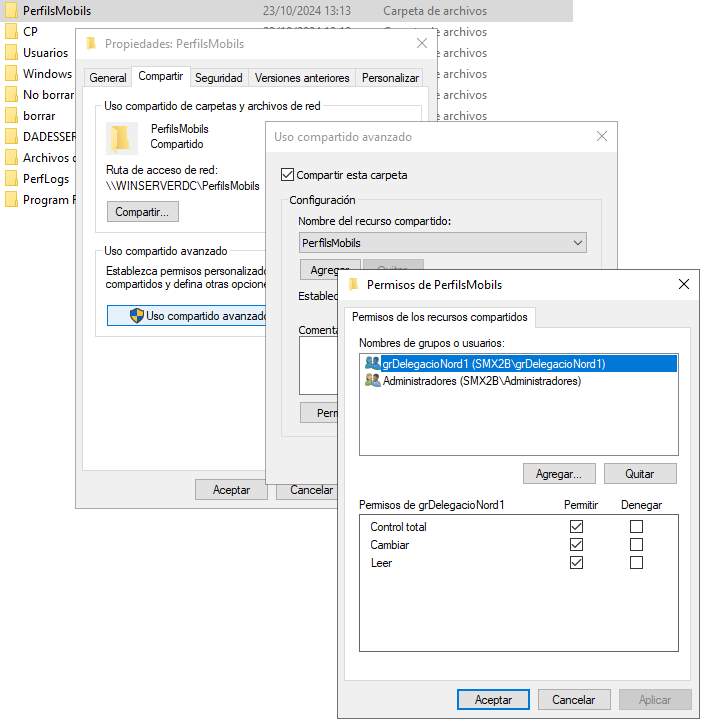
\includegraphics{png/CarpetaPerfilsMobils.png}
\caption{\emph{Figura1: Compartir una carpeta en el Servidor}}
\end{figure}

\subsubsection{Assignem la ruta del
perfil}\label{assignem-la-ruta-del-perfil}

En el \emph{dsa.msc} assignem el la ruta de la carpeta a un usuari
(Figura 2) Si seleccione, més d'un usuari (seleccionat amb Control)
podem fer-ho de colp amb la variable \textbf{\%username\%} (Figura 3)

\begin{itemize}
\tightlist
\item
  Per a un usuari podem usar el \emph{nom d'usuari} ( a la imatge usar
  la variable \%username\% )
\end{itemize}

\begin{figure}
\centering
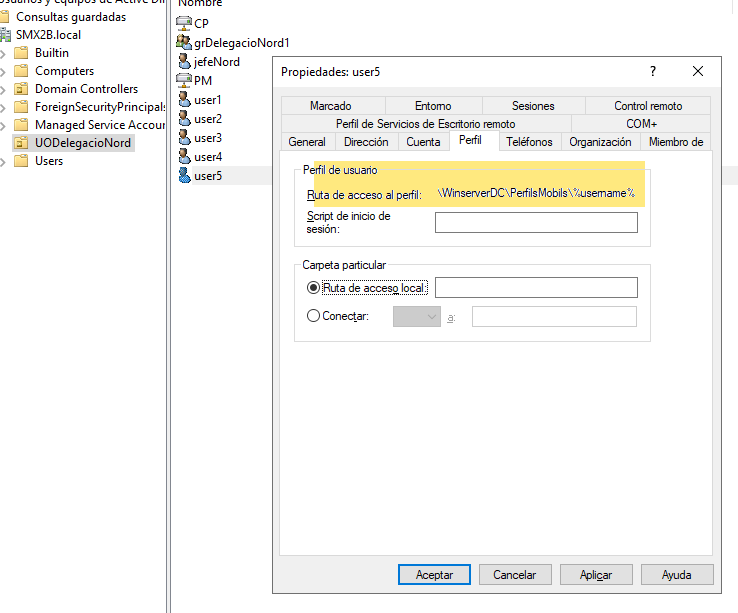
\includegraphics{png/RutaPerfils.png}
\caption{\emph{Figura2: Assignem la ruta del Perfi Mòbil a un usuari}}
\end{figure}

\begin{itemize}
\tightlist
\item
  Per a assignar a més d'un usuari al mateix temps ens valem de
  \%username\%
\end{itemize}

\begin{figure}
\centering
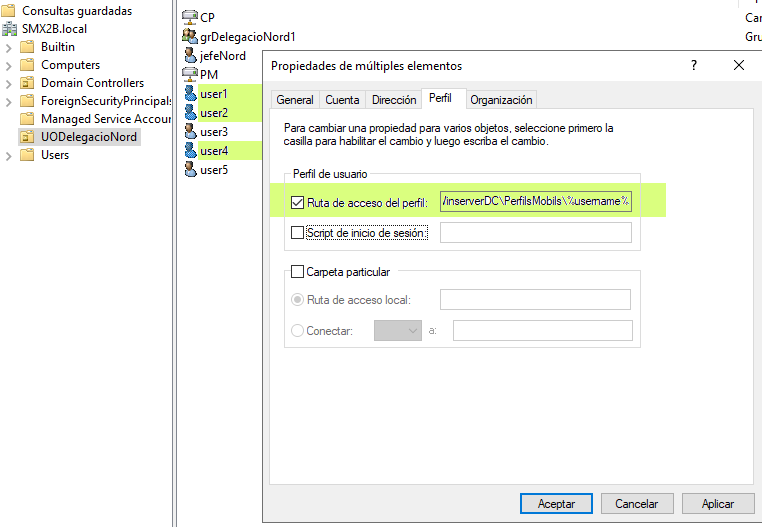
\includegraphics{png/RutaPerfils2.png}
\caption{\emph{Figura3: Assignem la ruta del Perfi Mòbil a más d'un
usuari}}
\end{figure}

\section{Carpetes particulars}\label{carpetes-particulars}

Son carpetes del Servidor que poden ser emprades per desar els treballs
de cada usuari a efecte de centralitzar els backups. Ací es tracta més
de dades del treball del dia a dia que de la confiuguració.

Ho fem de forma anàloga a l'anterior amb els usuaris que vullguem.

\begin{figure}
\centering
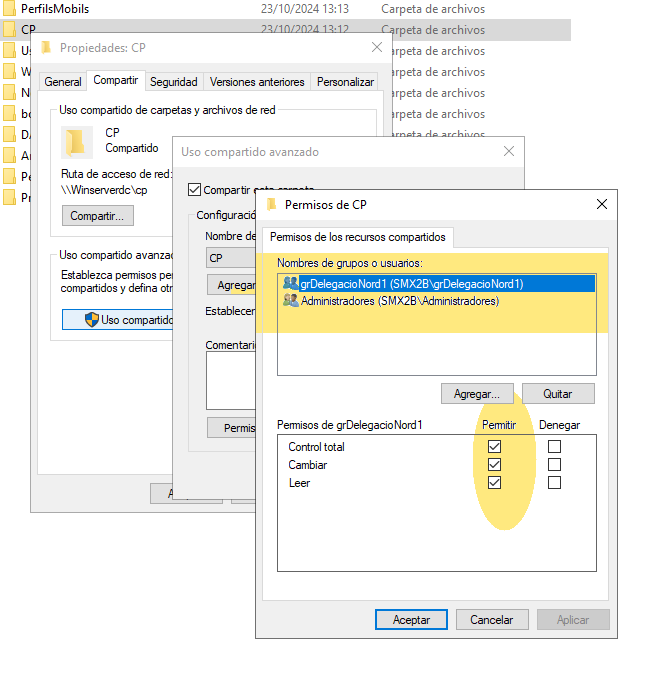
\includegraphics{png/CarpetaCarpetasParticulares.png}
\caption{\emph{Figura4: Compartir una carpeta en el Servidor}}
\end{figure}

\begin{figure}
\centering
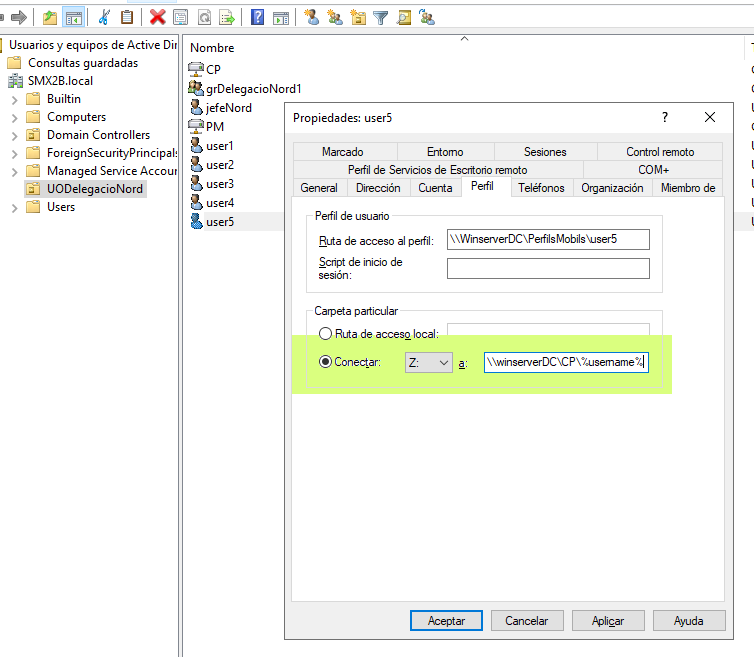
\includegraphics{png/RutaCarpetaParticular.png}
\caption{\emph{Figura5: Assignem la ruta de la Carpeta Particular a un
usuari}}
\end{figure}

També es pot aplicar a més d'un de colp amb \emph{\%username\%}

\begin{quote}
Nota

Moltes d'estes funcionalitats que estem aplicant de forma
individualitzada, més avant vorem que es poden (i deuen) fer de forma
més automatizada per atots els usuairs o PC de les UO o Domini. Ací és
on entren en joc els scripts amb cmdLets de PowerShell i les Directives
de grup.
\end{quote}

\section{Readreçament de carpetes}\label{readreuxe7ament-de-carpetes}

També és interessant que les carpetes habituals de treball com són
``Documentos'', ``Baixades'' etc. les puguem tindre guardades al
servidor i que també puga l'administrador del domini o l'operador de
backups fer una còpia d'elles.

\subsection{Crear la Directiva de
Grup}\label{crear-la-directiva-de-grup}

Ara treballarem en la consola de directives de grup: \textbf{gpmc.msc} (
\textbf{Administración de Directivas de Grupo})

Podem seleccionar la \textbf{UO (o el Domini sencer)} on volem que
s'aplique el nou adreçament. O crear la directiva i després vincular-la.

\begin{figure}
\centering
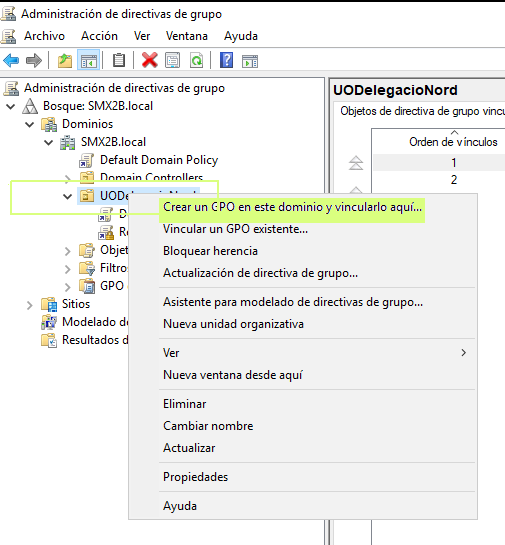
\includegraphics{png/CrearGPORedireccionar.png}
\caption{\emph{Figura6:Creem un nova directiva}}
\end{figure}

\begin{figure}
\centering
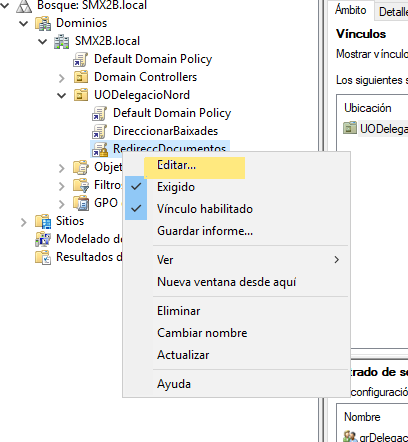
\includegraphics{png/EditarGPORedireccionar.png}
\caption{\emph{Figura7:L'editem}}
\end{figure}

\begin{figure}
\centering
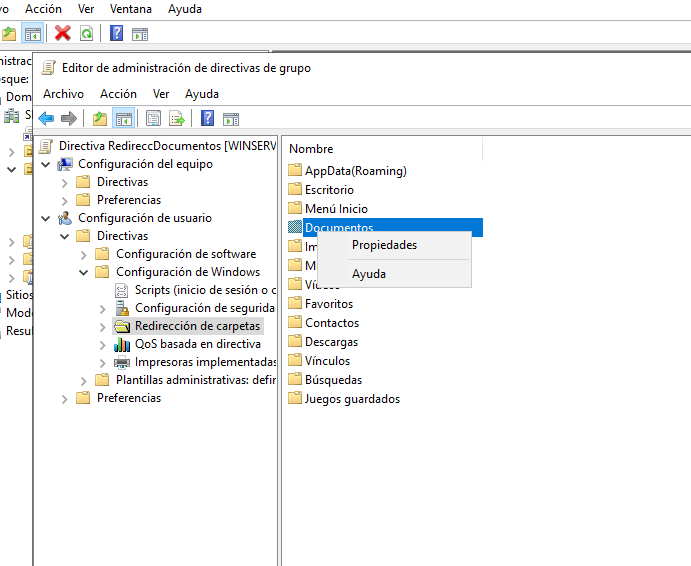
\includegraphics{png/PropiedadesGPORedireccionar.png}
\caption{*Figura8:Busquem en la plantilla el que volem modificar}
\end{figure}

\begin{figure}
\centering
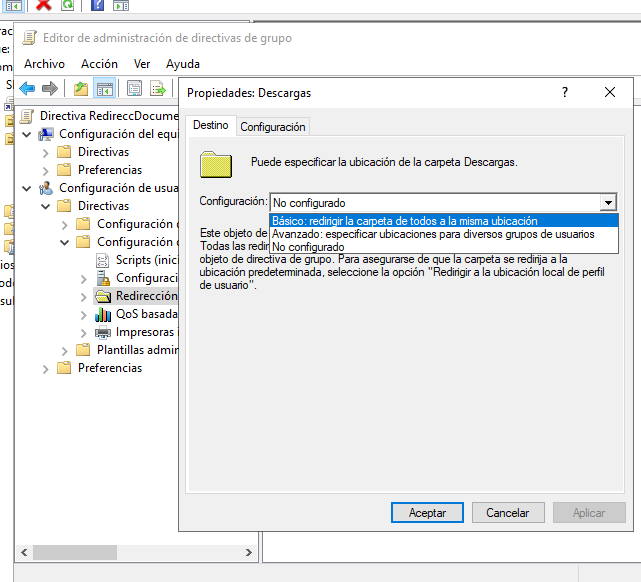
\includegraphics{png/Basico.png}
\caption{\emph{Figura9:Sols per a un grup: Básico}}
\end{figure}

\subsubsection{Una carpeta per usuari}\label{una-carpeta-per-usuari}

Independentment de la carpeta (Documents, Baixades\ldots), podem optar
per separar la informació de cada usuari.

Ací per crear una carpeta per cada usuari NO hem d'indicar el nom ni
\%username\%

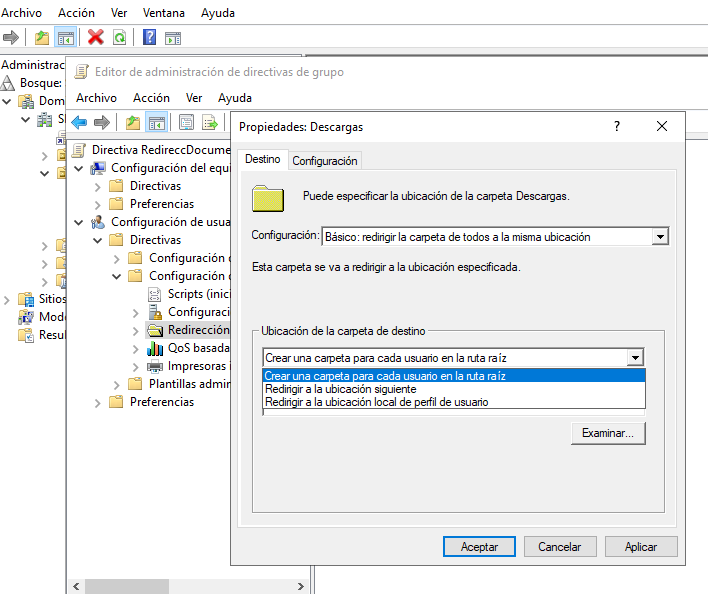
\includegraphics{png/CrearCarpeta.png}

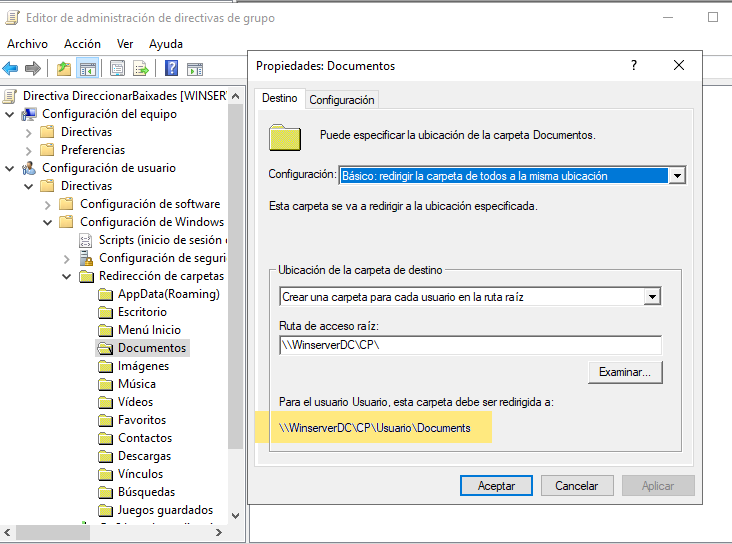
\includegraphics{png/CrearCarpetaRuta.png}

\subsubsection{Compartir tot en un sola
carpeta}\label{compartir-tot-en-un-sola-carpeta}

Independentment de la carpeta (Documents, Baixades\ldots), podem optar
per compartir en una sola carpeta.

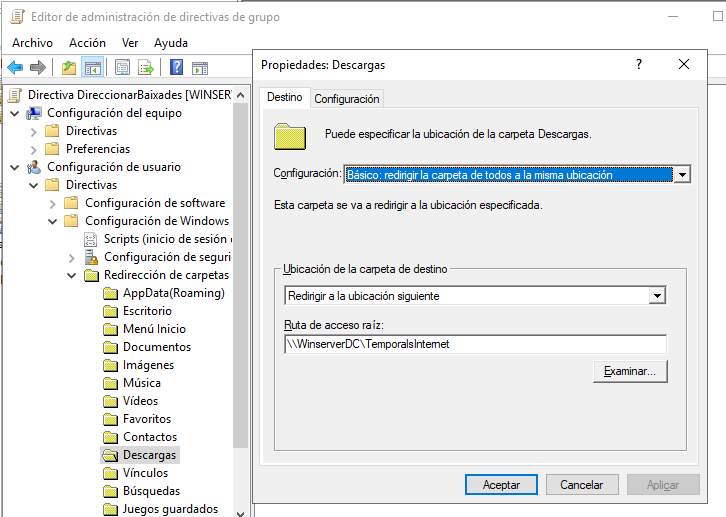
\includegraphics{png/CrearCarpetaRuta2.png}

\section{gpupdate}\label{gpupdate}

Recordeu:

\begin{Shaded}
\begin{Highlighting}[]
\NormalTok{gpupdate }\AttributeTok{/force}
\end{Highlighting}
\end{Shaded}

Si teniu iniciada la sessió d'un usuari tindreu este error:

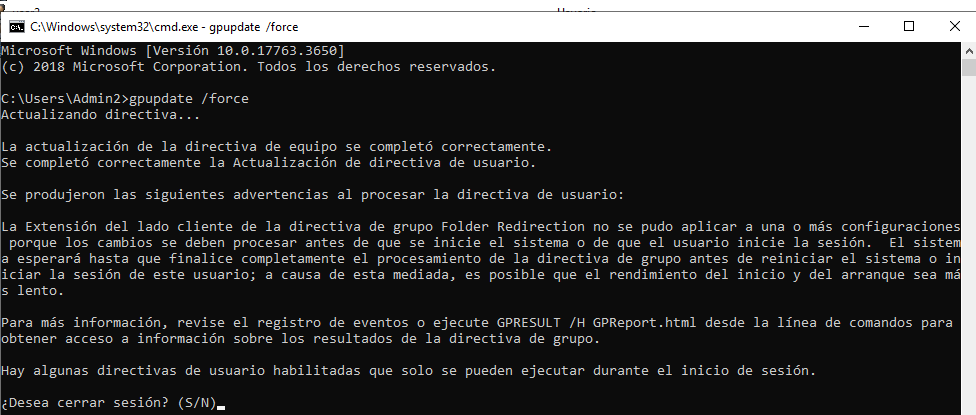
\includegraphics{png/gpupdateError.png}

Tanquem la sessió i repetim el \emph{gpupdate /force}

\section{Exemples d'ús}\label{exemples-duxfas}

Optem per carpetes particulars amb accès a través d'una unitat de xarxa
(P:) on cada usuari té una carpeta. Indiquem que no usen Documentos per
a informació de l'empresa. També podem ocultar la carpeta Documentos en
el client (com vàrem vore el curs passat en SOM).

Alternativament podem readrecem Documents a una carpeta compartida i no
usar les Carpetes Particulars.

O bé manteir les dos opcions. Carpeta Particular per a un tipus
d'informació i Documents per a altra.

Independentment, el Perfil pot ser o no mòbil.

\section{Consideracions finals}\label{consideracions-finals}

\subsection{Relació amb les Unitats Organitzatives
(UO)}\label{relaciuxf3-amb-les-unitats-organitzatives-uo}

El que hem vist es exemple d'utilitat de les Unitats Organitzatives.
Recordem que les UO són agrupacions d'objectes (usuaris, grups, altres
UO, carpetes\ldots) a efectes d'administració i transparents a l'usuari
final.

L'usuari guarda en ``Documents'' o en ``P:'' sense preocupar-se d'on ni
saber com treballa el company. Són els administradors qui han assegurat
que, encara que canvie de PC o es connecte amb un portatil al Domini,
sempre accedirà a les mateixes carpetes de dades i així controlaran
millor la còpia de seguretat o neteja de fitxers temporals.

\subsection{La solució depén del
cas}\label{la-soluciuxf3-depuxe9n-del-cas}

No existeix una forma ``correcta'' de configurar. Els administradors de
la xarxa han de tindre en compte les necessitats de l'organització, dels
usuaris i els seus costums per decidir:

\begin{enumerate}
\def\labelenumi{\arabic{enumi}.}
\item
  \textbf{Quina informació} convé desar al Servidor i fer \textbf{backup
  periòdicament} i quina pot quedar-se al PC Client per no tindre valor
  per a l'organització.
\item
  A partir d'ací, també hauran de marcar unes \textbf{normes d'ús} per
  als usuaris. Indicant-li on ha de guardar allò que és important per
  l'organització i on pot (si pot) deixar les ``seues coses'' o
  informació temporal sense valor. Es pot configurar que es guarde al
  Servidor, fins i tot, les descàrregues o altres fitxers temporals a
  efectes com hem vist.
\end{enumerate}

\end{document}
